\chapter{Introduction\label{ch:intro}}

Since the introduction of the Berry phase into the study of condensed matter physics, mathematical concepts such as Chern numbers and the Gauss-Bonnet theorem have been widely used in describing the topology of the momentum space of Bloch electrons in a crystal. This theoretical advance has resulted in new ways to describe, classify and study the solids. Such classification typically leverages a topological order that depends on the integration of Berry curvatures in the whole Brillouin zone instead of only focusing on the local property of the wave function. As a result, many novel phases of matter have been found such as topological insulators, Chern insulators, Dirac semimetals and Weyl semimetals. These new classes of matter not only provide us a new perspective to view the crystals, but also can be used to imitate some mysterious phenomena in high energy that has been under search for a long time, such as axion electrodynamics, Majorana fermions, and the chiral anomaly effect. In addition, these new concepts could be of great value in applications. For example, the dissipationless edge states in of a Chern insulator have been proposed to construct the conducting channels in future integrated circuits to solve the Joule heating problem in the conducting wires. Besides, there are many theoretical proposals that leverage Majorana fermions built from TIs to form the quantum bit of a topological quantum computer in the future. Such applications will need a complete and detailed experimental study of the topological materials. In this introduction, we will briefly introduce both the theoretical and experimental progress in the investigation of TI, DSM and WSM in recent years. Then in later chapters we will describe the progress we have made in this area in the last few years.

%add formula for Berry phase, citations needed.

\section{Topological Insulators}
\label{sec:intro:TI}


The idea of describing the physical properties of crystals with topological concepts comes from the development of understanding the quantum Hall effect (QHE). Discovered by Klaus von Klitzing~\cite{Klitzing1980}, the Hall signal of a high-mobility two-dimensional electron gas (2DEG) at low temperatures displays plateaus at $\sigma_{xy}=ne^2/h$ (where $h$ is the Planck constant) when a strong magnetic field is applied. Such plateaus happen when the two-dimensional (2D) Fermi energy $E_F$ lies between the quantized Landau levels (LLs). Although there are no itinerant states in the gap between the Landau levels in the 2D bulk, the increasing LL energy at the edge caused by the surface potential leads to states intersecting the Fermi level. Since such edge states cannot be scattered into the bulk, they provide dissipationless chiral channels for the electrons. The theoretical advances thereafter then showed that each LL in QHE has a Chern number $\nu=1$ and it lead to the development of the topological band theory. Thus QHE provides an important early example for the necessity of topological orders in describing properties of Bloch electrons.

Both the QHE and the later discovered fractional quantum Hall effect (FQHE) only exist in a strong magnetic field when the TR symmetry is broken. Then a question arises as whether the similar states could exist without a magnetic field. In 1988, the pioneering work by Haldane~\cite{Haldane1988} constructs such a model without breaking the time reversal symmetry (TRS) globally. But this model still needs a local magnetic field that points up and down at different sites. Enlightened by Haldane's work, Zhang et. al.~\cite{Bernevig06} found in 2006 that the spin-orbit coupling (SOC) could play the role of the flipping magnetic field in real solids. They also predicted that the HgTe/CdTe quantum well could be an example of the model and it was later realized experimentally by Molenkamp group~\cite{Konig2007}. This becomes the first example for the 2D TI and it's also called quantum spin Hall effect (QSHE). 


%here needs better explanation and a figure
A simple picture of QSHE is to view it as two stacking sets of QHE with counter-flowing edge states (Fig. \ref{QSHE}). The QSHE thus has two edge states which form the time-reversal partner of each other. Since the spin of the edge state is locked to its momentum in QSHE, such edge channel lacks the 2$k_F$ scattering and it leads to the quantized conductivity in Ref ~\cite{Konig2007}. Since the 2$k_F$ scattering usually contributes a significant amount to the scattering processes in transport experiments, an electric device based on QSHE is predicted to produce less Joule heating due to the decreased scattering. 
%A key player in realizing the quantum spin Hall phase is the band inversion induced by the SOC in HgTe, which later also plays a critical role in generating the 3D TIs. 
\begin{figure}[htb]
  \begin{center}            
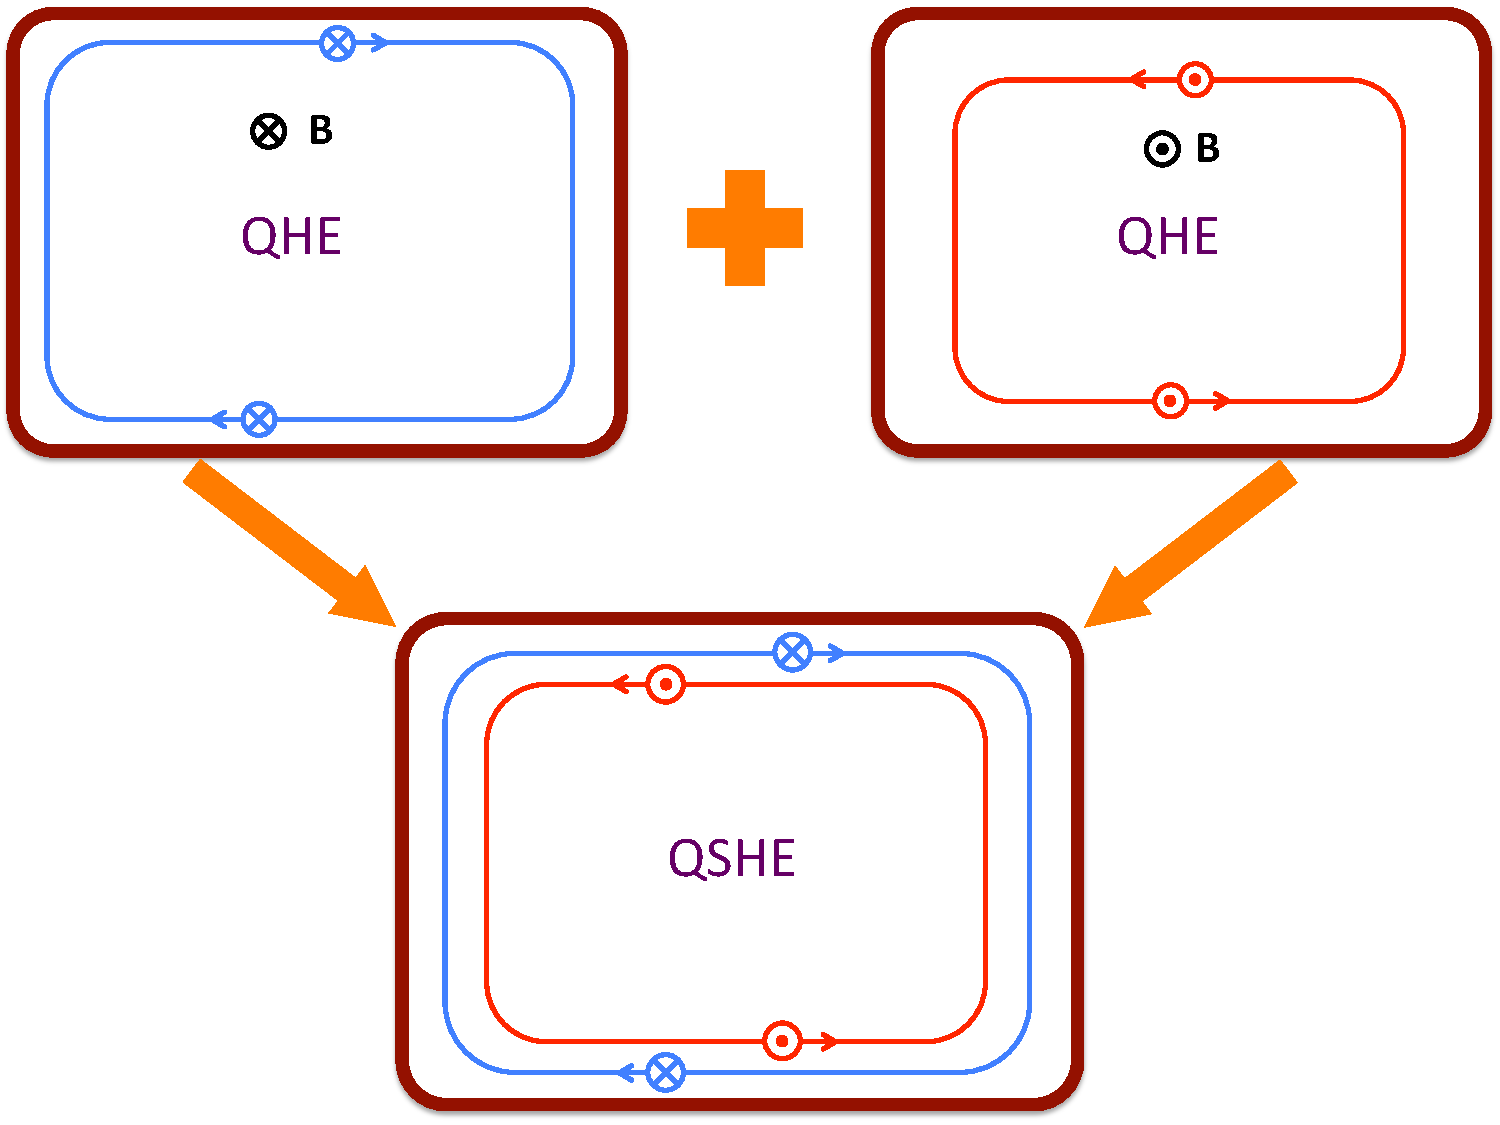
\includegraphics[width=0.9\linewidth]{ch-intro/figures/QSHE.pdf} 
\caption{\label{QSHE} (Color online) 
The edge states in quantum spin Hall effect can be viewed as a stack of two quantum Hall edge states with opposite directions.
} 
  \end{center}
\end{figure}

An important progress later is to extend the topological band theory to the 3D case. In 2007, Fu and Kane~\cite{FuKane07, Fu07} successfully made this step and found the theoretical ingredients for 3D $Z_2$ TIs. They found that four $Z_2$ topological invariants $[\nu_0; \nu_1, \nu_2, \nu_3]$ could be used to classify the different topological properties of a crystal. Within these four numbers, $[\nu_0]$ is the strong topological invariant, which is also the most important one that defines a strong or weak TI. $[\nu_1, \nu_2, \nu_3]$ are called weak topological invariants, and could be used to classify different weak TIs. Fu and Kane~\cite{FuKane07} used the pfaffians at the Kramers points inside the first Brillouin zone to calculate $[\nu_0]$ as the following:
\be
(-1)^{\nu_0}=\prod \delta_a, 
\label{eq:nu0}
\ee
where $\delta_a = Pf[\omega(\Lambda_a)]/\sqrt{Det[\omega(\Lambda_a)]} = \pm1$. Here $Pf[\omega(\Lambda_a)]$ is the pfaffian, and the $
\omega$ matrix is $\omega_{mn}(\bf k) = \Braket{u_{m -k}|\Theta|u_{nk}}$, where $\Theta$ is the time reverse operator. As a result, a 
conventional trivial insulator has topological invariants $[\nu_0; \nu_1, \nu_2, \nu_3] = [0, 0, 0, 0]$. For a strong TI, $\nu_0=1$. A weak TI has $\nu_0=0$ but at least one of the weak topological invariants is non-zero.

\begin{figure}[htb]
  \begin{center}            
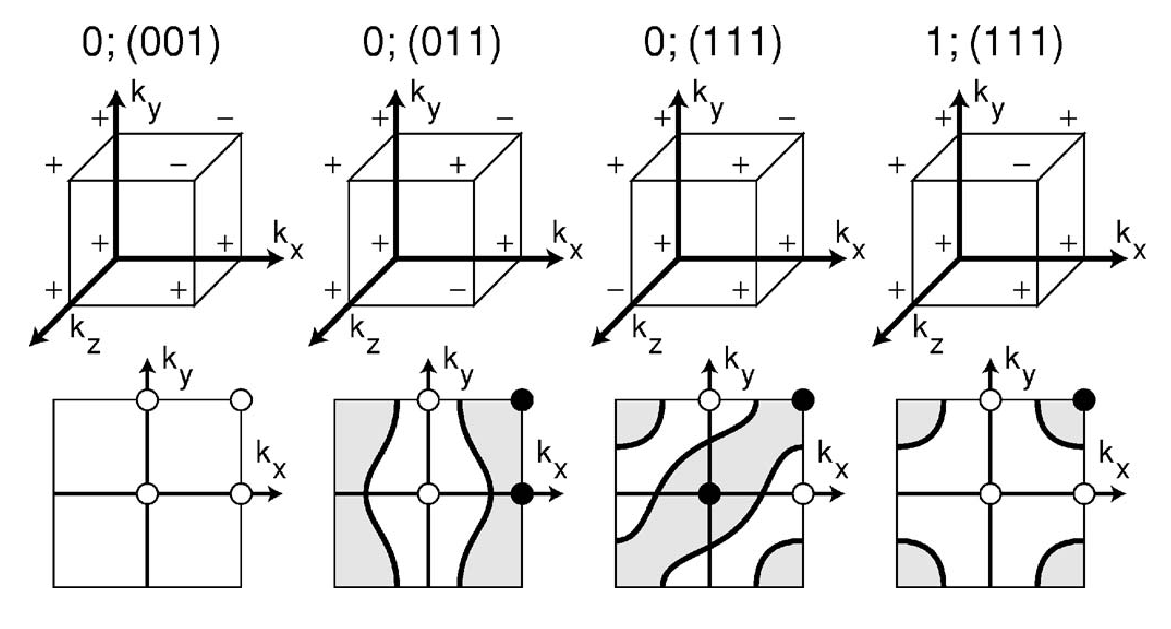
\includegraphics[width=0.9\linewidth]{ch-intro/figures/TI_class.pdf} 
\caption{\label{TI_class} (Color online) 
The four diagrams give examples of different types of weak and strong TIs. The top panels depict the signs of $\delta_i$ at the Cramers points $\Lambda_i$ in the reciprocal lattice. The bottom panels display the corresponding surface states.
} 
  \end{center}
\end{figure}

Same as the earlier found topological phases, a 3D TI also has metallic states on its edge, the 2D surface, while its 3D bulk is an insulator. These surface states also provide an easy way to distinguish strong TIs, weak TIs and trivial insulators in experiments. Fu and Kane pointed out that on the surface of a strong TI, there is an odd number of states connecting the bulk conduction band and the valence band. These surface states, which exist on every plane cleaved out of the crystal, are robust because they cannot be destroyed by local perturbations from the impurities. However, weak TIs only have some robust surface states on certain cleavage planes. By contrast, a trivial insulator do not have such robust surface states at all. Besides, one important property of the surface states on a strong TI is the spin-orbit lock-in effect. Thus, the spin direction of the surface state is always perpendicular to both the wavevector $\bf k$ and the surface normal vector $\bf{\hat{n}}$.

The prediction of the spin-polarized surface states on 3D TI has largely expanded the scope of possible experiments on the topological properties of solids. Most of the experiments are focused on strong TI, and there has been important progress in experiments with techniques like angle-resolved photoemission spectroscopy (ARPES), scanning tunneling microscopy (STM) and transport measurement. The first experimental discovery of a 3D TI is the ARPES result on Bi$_{1-x}$Sb$_x$ by Hasan's group \cite{Hsieh08, Hsieh09}. As shown in Fig. \ref{ARPES_STM}A, there are five surface bands inside the bulk band gap. The spin ARPES data showed that these surface states indeed are spin-polarized. Then more ARPES experiments found that Bi$_2$Se$_3$ and Bi$_2$Te$_3$ \cite{Xia09, Chen09} are also strong TIs but they have a much simpler surface band structure. As shown in Fig. \ref{ARPES_STM}B and D, both Bi$_2$Se$_3$ and Bi$_2$Te$_3$ only have one surface state across the bulk band gap. Since these surface states have a linear dispersion to the first order, they could be described by the Dirac equation and are also called Dirac surface states. They are also a good analog to the Dirac states in graphene. STM experients by Yazdani group\cite{Pedram09} have also confirmed the lack of back-scattering of the topological surface states. 

\begin{figure}[htb]
  \begin{center}            
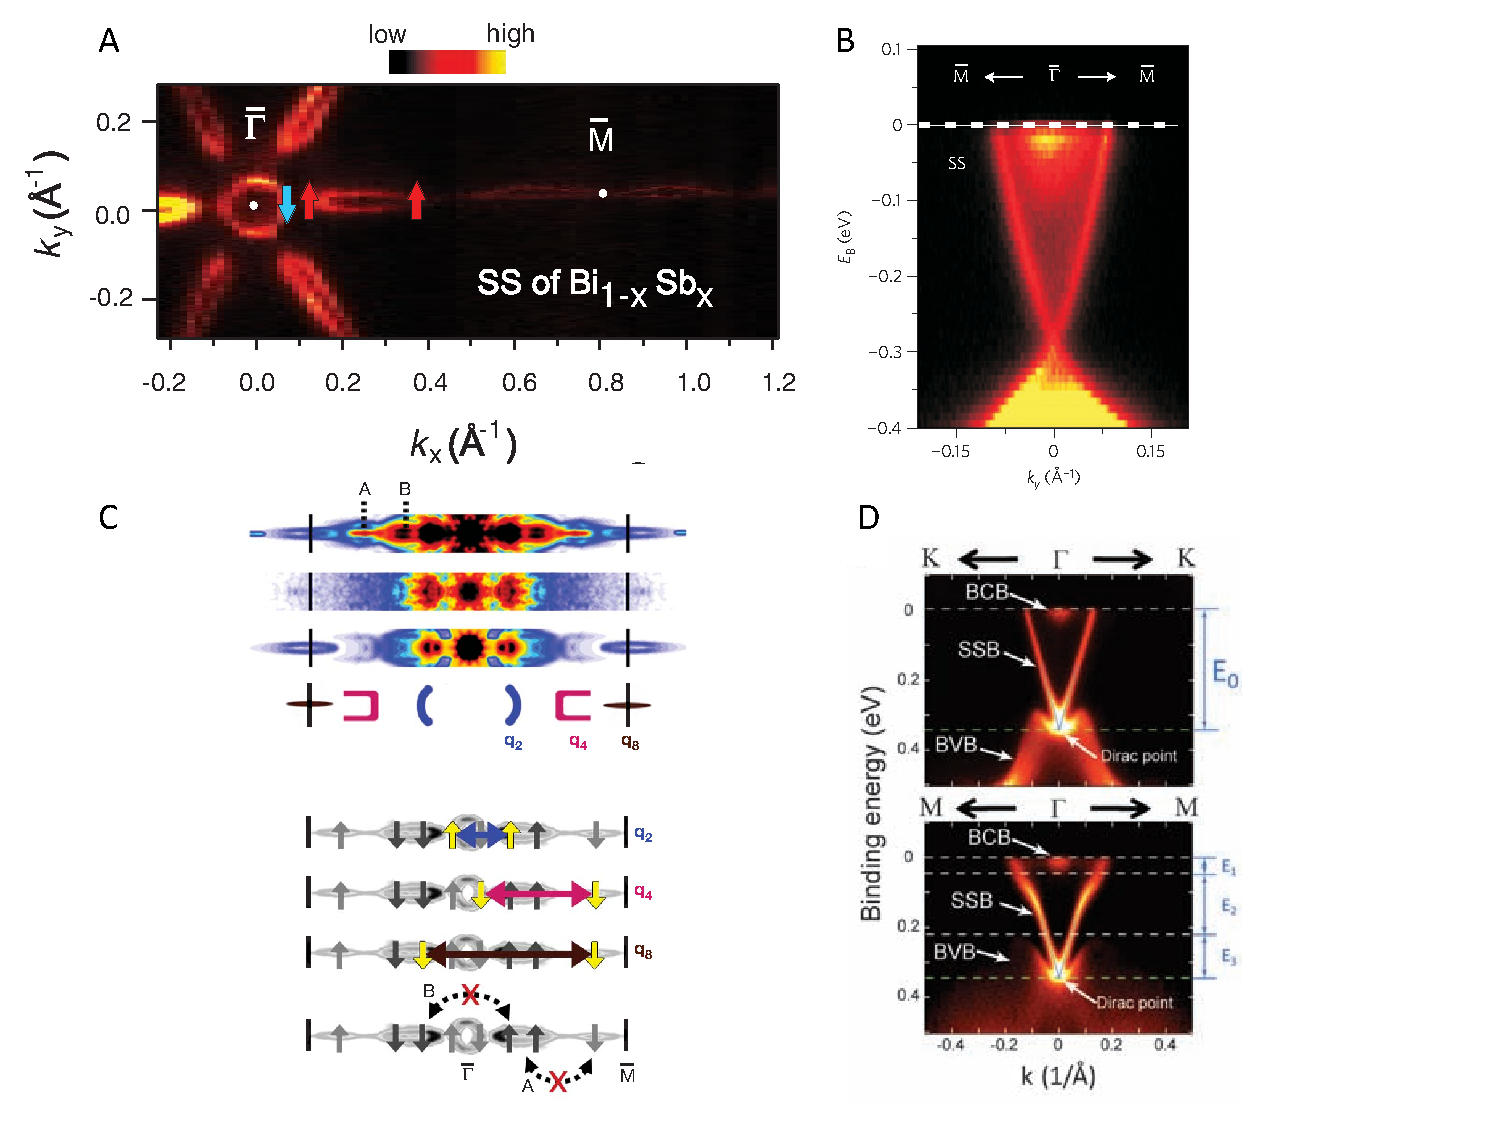
\includegraphics[width=0.9\linewidth]{ch-intro/figures/ARPES_STM.pdf} 
\caption{\label{ARPES_STM} (Color online) 
The first ARPES and STM results on some topological insulators. (A) The ARPES experiment on the first example of a strong TI, Bi$_{1-x}$Sb$_x$, indicates five spin-polarized surface states at the Fermi level\cite{Hsieh09}. (B) The ARPES data on Bi$_2$Se$_3$ shows a single surface cone with a 0.3 eV bulk energy gap \cite{Xia09}.  (C) The quasiparticle interference results in an STM experiment on Bi$_{1-x}$Sb$_x$ confirms the lack of back-scattering of the topological surface states. (D) The ARPES data on Bi$_2$Te$_3$ gives another example of a TI with a single surface cone and a large bulk energy gap \cite{Chen09}.
} 
  \end{center}
\end{figure}

Despite the fast advances in experiments using surface-sensitive techniques, the transport measurement of a TI's surface states have been difficult, mainly due to the vast amount of carriers in the bulk. Unexpected by the theory, the inverted bulk band gap induced by the SOC in TIs may still have a lot of states inside. The reason is that the crystal defects and imperfection in real TI crystals can easily dope the materials and make the as-grown crystals $n$-type (Bi$_2$Se$_3$) or $p$-type (Bi$_2$Te$_3$). Besides, the surface states are still vulnerable possibly due to the chemical reaction that happens when the sample is exposed to air. Hence, the surface states typically contribute only to a small portion of the total current, and thus are hard to detect in transport experiments. Despite the difficulty, Qu et. al. ~\cite{Qu} and Analytis et. al. ~\cite{Analytis} found the first convincing transport signals for the surface states on TI in Bi$_2$Te$_3$ and (Bi$_{1-x}$Sb$_x$)$_2$Se$_3$. These experiments have triggered enormous interest in the transport experiments on TIs. And we will discuss our progress in the transport investigation of TIs in later chapters. 

\begin{figure}[htb]
  \begin{center}            
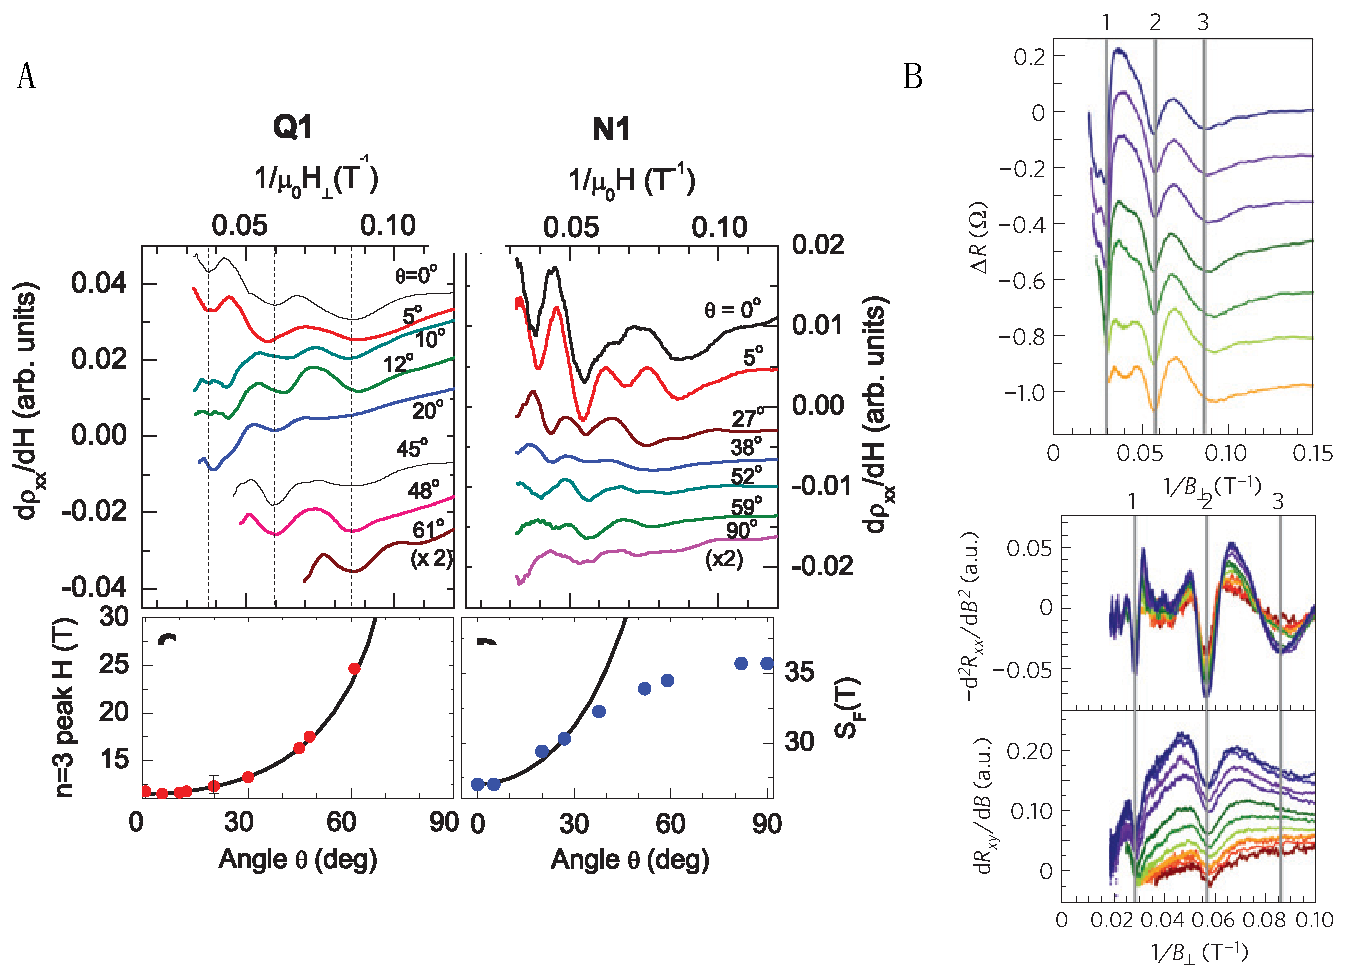
\includegraphics[width=0.9\linewidth]{ch-intro/figures/TI_transport.pdf} 
\caption{\label{TI_transport} (Color online) 
Quantum oscillations at high magnetic fields confirm the existence of high-mobility surface states on TI. (A) The different angle dependences of the quantum oscillations in nonmetallic and metallic Bi$_2$Te$_3$ samples indicate the surface origin of the quantum oscillations in nonmetallic samples. (B) Quantum oscillations in the magnetoresistance data of (Bi$_{1-x}$Sb$_x$)$_2$Se$_3$ are consistent with the behavior of surface states when the magnetic field is tilted.
} 
  \end{center}
\end{figure}



\section{Weyl and 3D Dirac Semimetals}
\label{sec:intro:Weyl}
%1 chiral
%2 from Berry phase to chiral charge
%3 current between the Weyl nodes
%4 poor man�s approach for chiral pumping
%
%experimental progress, ARPES (including Fermi arcs), transport
%
%
%
%Besides the progress in TI, interesting concepts of Weyl semimetals and 3D Dirac semimetals have also been developed.

While the surface states on TI provide an analog to the 2D Dirac electrons in graphene, interesting concepts of Weyl semimetals and 3D Dirac semimetals were also developed as examples of 3D Dirac electrons. With a linear energy-momentum dispersion, both Weyl semimetals and Dirac semimetals can be viewed as 3D analogs of the 2D graphene. Besides, Weyl semimetals provide a solid-state realization of the Weyl fermions that have been studied theoretically for a long time in high energy physics. Weyl fermions are a type of massless fermions with handedness, i.e. chirality. The chirality describes whether a particle spins clockwise or anti-clockwise when viewed in front of the traveling direction. In absence of an electromagnetic field, the chirality of each Weyl fermion is conserved. Therefore, a Weyl fermion cannot shift its handedness without the combination of the electric and magnetic fields. In a 3D crystal, Weyl fermions can be imitated by quasiparticles of electrons with the Hamiltonian as the following:
%\be
%H_{\pm}=\pm \nu_F (p_x \sigma_1 + p_y \sigma_2 + p_z \sigma_3),
%\label{eq:H_W}
%\ee
\be
H=\bf p \cdot \bf V \cdot \pmb{\sigma},
\label{eq:H_W}
\ee
where $\bf V$ is the velocity matrix, $\bf p$ is the electron's 3D momentum vector deduced by the Weyl nodes in the Brillouin zone, and $\pmb{\sigma} = (\sigma_x, \sigma_y, \sigma_z)^T$ denotes the vector formed by the three Pauli matrices. If a Weyl node is at $\bf{k_W}$ in the reciprocal space, then $\bf p= \hbar (\bf k-\bf k_W)$, where $\bf k$ is the electron's wavevector. The Pauli matrices $\sigma_i$ (i = x, y, z) live in the space spanned by the pair of bands that touch at the Weyl nodes. Here each of the two bands is single-degenerate. Thus the system could not respect time reversal and inversion symmetry simultaneously. The above equation shows that the chirality in the Weyl semimetal is formed by the electron's momentum and its peudospin described by the Pauli matrices. Then the chirality of the system is $\chi = sign(det(\bf V))$, which could be $\pm 1$ for the left-handed and right-handed Weyl fermions respectively. As in the case of high-energy Weyl fermions, the Weyl nodes in a crystal always appear in pairs with opposite chiralities. The crystal whose low energy dispersion could be described by Eq.\ref{eq:H_W} near a Weyl node is called a Weyl semimetal.

In addition, we may also have a pictorial understanding of the Weyl nodes and their chiralities from the perspective of the Berry phase. A Bloch 
electron moving inside the Brillouin zone feels the Berry vector potential $\bf A(\bf k) = i \Bra{u(\bf k)}\bf \nabla_{\bf k} \Ket{u(\bf k)}$. This vector potential yields the Berry field $\bf F(\bf k)=\bf \nabla_{\bf k} \times \bf A(\bf k)$ that deflects the direction of Bloch electrons in the momentum 
space. $\bf F(\bf k)$ is also called the Berry curvature or the Chern flux. Thus $\bf F(\bf k)$ acts as a magnetic field that bends the momentum trajectory of a moving electron in a crystal. In a WSM, the chirality $\chi$ of a Weyl node can be calculated by the total Berry flux through an enclosing surface with the following equation:
\be
\frac{1}{2\pi}\oiint\limits_{FS} \VF{F(k)} \cdot \dif{\VF{S(k)}}=\chi, 
\label{eq:chi_Berry}
\ee
where the integral is over the whole Fermi surface that encloses the Weyl node. This equation suggests that a Weyl node acts as a monopole that generates the Berry curvature in the momentum space. Weyl nodes with opposite chiralities are similar to magnetic monopoles with opposite magnetic charges. Besides, since $\bf F(\bf k)$ is the Chern curvature, the above equation indicates that a Fermi pocket that encompasses a Weyl node has a non-trivial Chern number $\chi$.

In a crystal with both time reversal symmetry and inversion symmetry, such separated Weyl pairs do not exist because the bands involved are always degenerate. When two Weyl nodes with opposite chiralities meet in a crystal, they generally annihilate and open a band gap. However, Wang et. al.~\cite{Wang2012, Wang2013}  found that with certain crystal symmetries, paired Weyl nodes can overlap in the momentum space and it results in a new crystal with a linear energy-momentum dispersion, namely a 3D Dirac semimetal. Unlike a WSM, a 3D Dirac crystal respects time reversal and inversion symmetries at the same time. Besides, 3D Dirac cones also accidentally exist in many solids. For example, at the phase transition between a topological insulator and a trivial insulator, the conduction and valence bands of the crystal touch and form a linearly dispersed Dirac cone. However, such accidentally formed Dirac semimetals are not stable since they need fine tuning of chemical compositions and a small perturbation may open a gap at the Dirac point. Nevertheless, the DSMs found by Wang et. al. ~\cite{Wang2012, Wang2013}, i.e. Cd$_3$As$_2$ and Na$_3$Bi, are robust against small perturbations due to the protection by the crystal symmetries. Wang et. al. also predicted the existence of the surface Fermi arcs that connect different Dirac points. Their predictions have been confirmed by ARPES experiments~\cite{Liu2014a, Xu2015, Liu2014, Neupane2014}. Thus such crystals become the maternal materials for Weyl semimetals. Later, Weng et. al. ~\cite{Weng2015} and Huang et. al. group ~\cite{Huang2015} predicted a series of Weyl semimetals that lack inversion symmetry, such as TaAs and NbAs. In these crystals, the Weyl nodes are already separated due to the lack of the inversion symmetry. They also predicted Fermi arcs on the surface that connect the bulk Weyl nodes.Then these findings were confirmed by ARPES experiments~\cite{Xu2015}.

Besides the value in the theoretical aspect, Weyl semimetals also have very interesting transport properties. One of them is the chiral anomaly effect that pumps charges from one Weyl branch to its pair in the presence of an electromagnetic field. A simple picture to understand the chiral anomaly effect in a Weyl semimetal is as the following. If we suppose that the Weyl fermion has entered the lowest Landau level (LL) in a strong magnetic field. The energy dispersion for the $n=0$ Landau level is $\varepsilon_0 = -\chi \hbar \nu_F \VF{k \cdot \hat B}$, where $\hbar$ is the Planck constant and $\VF {\hat B}$ is the normal vector of the magnetic field. We suppose that both the temperature and the chemical potential are low (smaller than $\nu_F \sqrt{\hbar eB}$). Also, the degeneracy of one Landau level formed by one Weyl node is $g = \frac{B S}{h/e}$, where $S$ is the cross-section of the sample that is perpendicular to $\bf B$. If an electric field $\bf E$ is also applied on the same direction as $\bf B$, the states in the momentum space will move according to $\hbar \VF{\dot{k}}=-e  \VF{E}$. Thus the charge pumping rate between Weyl nodes with opposite chiralities is $\VF{\dot{Q}} = e \chi g L |\VF{\dot{k}}|/2\pi=-e^2 \chi g L|\VF{E}|/h$, where L is the length of the crystal along the $\bf B$ direction. Putting in the expression for the degeneracy of the lowest Landau level, we obtain the charge pumping rate for unit volume:
\be
\VF{\dot{Q}}= -\frac{e^3}{4\pi^2\hbar^2} \VF{E} \cdot \VF{B}
\label{eq:chg_pmp}
\ee

%Although we only showed the correctness of the above formula in the case of the lowest LL and when $\bf B$ and $\bf E$ are parallel, strict calculations (cite) have shown that this formula is concrete even more LLs are occupied when $\bf B$ and $\bf E$ are not parallel. 

Although it seems to annhilate or create charges for one Weyl branch, the pumping effect does not violate the charge conservation law in a crystal because Weyl nodes with opposite chiralities always appear in pairs. The above charge pumping effect is also called Adler-Bell-Jackiw chiral anomaly, which was originally used to explain the neutral pion decay in particle physics. Thus the WSM provides us an opportunity to study the chiral anomaly phenomenon in high energy physics.

\begin{figure}[!htbp]
  \begin{center}            
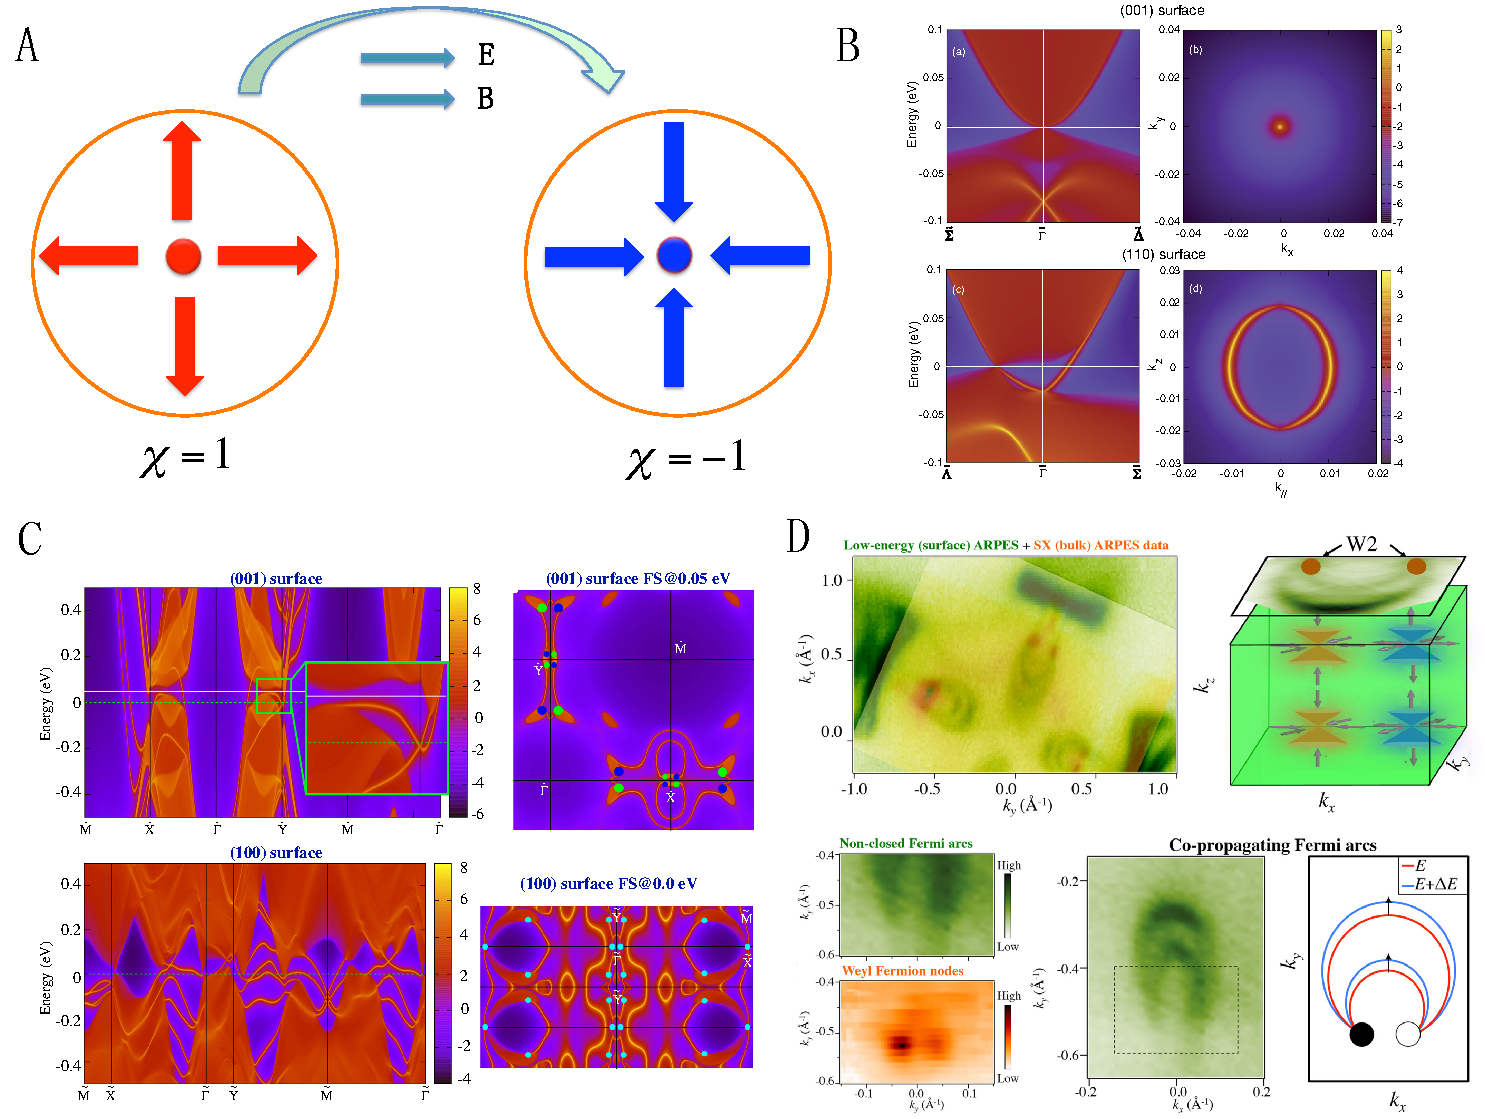
\includegraphics[width=0.9\linewidth]{ch-intro/figures/WeylDirac.pdf} 
\caption{\label{QSHE}
The Weyl and Dirac nodes of Weyl semimetals and Dirac semimetals. (A) The paired Weyl nodes are opposite monopoles of the Berry curvature. In an electric-magnetic field, charges are pumped between the Weyl nodes. (B) The predicted Dirac node and surface Fermi arcs of the Dirac semimetal Cd$_3$As$_2$~\cite{Wang2013}. (C) The predicted multiple Weyl nodes and the surface Fermi arcs that connect them in the Weyl semimetal TaAs~\cite{Weng2015}. (D) ARPES experiments by Hasan's group confirmed the surface Fermi arcs on TaAs~\cite{Xu_TaAs}.
} 
  \end{center}
\end{figure}

